\documentclass{article} %document style and layout
\usepackage[table, dvipsnames]{xcolor} %colors for tables and text
\usepackage{graphicx} %to insert images
\graphicspath{ {./Images/} }
\usepackage{tabu} %creation of tables
\usepackage{array}
\usepackage{enumitem} %list of elements
\usepackage{hyperref} %insert clickable links
\urlstyle{same}
\usepackage{subfig} 
\setcounter{lofdepth}{2} %subfig used to have more than 1 figure together, \setcounter used to add subfigures in the list of figures
\usepackage{float}



%-------Titlepage information------------------------------------------
\title{\textbf{\huge{PAPS: A first step into the implementation phase. Partitioning a network.}}}
\author{\color{black}Fabio Losavio, Oscar Francesco Pindaro \\ \\
        Dipartimento di Elettronica, Informazione e Bioingengeria \\
        Politecnico di Milano, Italy \\
        \texttt{\{fabio.losavio,oscarfrancesco.pindaro\}@mail.polimi.it}}
\date{xx - May - 2020}
%------------------------------------------------------------------------


%DOCUMENT BEGINNING
\begin{document}
%TITLEPAGE and ABSTRACT
\maketitle

\begin{abstract}
    The emergence of latency-sensitive and data-intensive applications requires to move the 
    computational power closer to users on nodes at the edge of the network (\textit{edge computing}).
    This work starts from PAPS \cite{PAPS}, a framework which aims to tackle the complexity of edge 
    infrastructures by means of decentralized self-management and serverless computing. This paper
    shows how the first of the four PAPS phases, \textit{partitioning}, is implemented and integrated
    with a common open-source system: Kubernetes \footnote{Kubernetes website: https://kubernetes.io/},
    to easily deploy the system in an already
    existing network. The partitioning is mainly focussed on the division of the network in multiple 
    communities in order to reduce the scope of the following parts. The division is performed using 
    the SLPA \cite{SLPA} algorithm, which uses a label spreading technique to assign each node to a
    community. Once all the nodes are assigned, the Kubernetes node will be modified using the API 
    labeling it in order to easily recognize and manage each community.
    \\ \\
    \textbf{Keywords:} Edge computing \textbf{\textperiodcentered} Partition 
    \textbf{\textperiodcentered} Kubernetes \textbf{\textperiodcentered} PAPS
    \textbf{\textperiodcentered} Community division \textbf{\textperiodcentered} SLPA
    
\end{abstract}
%------------------------------------------------------------------------------------------------------------------------------------------------
{{\section{Introduction}\label{sect:intro}}}
PAPS is an edge computing framework which aims to improve network performances of some 
applications moving the computation closer to the final user instead of doing that on 
a centralized server. This will reduce the amount of traffic flowing into the network
with the result of an improvement of the throughput allowing to better meet the SLAs
of delay sensitive applications.

This framework focuses on MEC topologies, composed of geo-distributed nodes which access
the system through cellular base stations. In a typical topology is possible to identify
two different networks: the \textit{fronthaul network}, which connects normal nodes to 
the MEC stations, and the \textit{backhaul network}, which interconnects the MEC stations.
PAPS aims to reduce the complexity of the problem working at three different levels: 
\textit{system, community and node}. 
\\
\subsubsection*{System level}
Since MEC topologies can be really big and complex, the first step is to \textit{partition}
the network in multiple delay-aware sub-networks called \textit{communities}. Each community
is composed by a set of nodes whose propagation delay from one another is below a given 
threshold. PAPS assumes the availability of a \textit{supervisor} that has a global view of
the MEC topology and uses SLPA \cite{SLPA} to create the communities. Each community will
elect a \textit{leader} which will be in charge of managing the community and the communication
between the nodes.

\subsubsection*{Community level}
Communities aims to minimize the likelihood of of SLA violations so that the MEC nodes
can operate under feasible conditions.\\
Each community leader will manage the \textit{allocation and placement} phases by looking at 
the aggregate demand to each service and the node capacities in order to decide how to 
distribute resources among the nodes in its community. This is done solving a \textit{mixed
integer programming (MIP)} problem whose goal is to minimize the overall community delay. 
The MIP is solved periodically by the community leader which will then contact the other members
to communicate the new configuration.

\subsubsection*{Node level}
The Node-Level Self-Management system aims to keep the response time for a given function fixed, 
by deploying and removing containers accordingly to the measured workload.
In order to achieve this, every node has a controller for each function that is hosting; all the controllers
run in parallel and independently.
Each controller accepts as input the number of container allocated for its function and the 
measured arrival rate, and outputs the response time. The objective is to keep the response time
at the control set point, which must be lower than the SLA.




%------------------------------------------------------------------------------------------------------------------------------------------------
{{\section{PAPS}\label{sect:paps}}}
 %Ricontrollare come è scritto, magari aggiungere qualcosa di discorsivo
 %mettere immagini
As already said, the importance of edge computing is growing, because some applications can not 
deal with the high latency from devices to cloud data centers.
In this context, the way in which applications are allocated and distributed on
edge nodes is crucial in order to have high performance and respect the SLA requirements
of these applications.
\\
At the same time, serverless computing is a new cloud computing paradigm that is becoming more
and more popular, since it allows the developer to focus on the development of an application
while ignoring the infrastructure on which the function will be deployed.
\par
PAPS is a framework that tries to tackle the challenges related to the management of edge computing infrastructures.
\\
Its main objective is to automate the allocation of serverless function and the management of large scale edge topologies.
It should be able to give an optimal allocation for a given workload, but also
to react to unpredictable workload fluctuations that characterize this type of networks.
%----------------------------- SONO INDECISO SE TENERE STA PARTE ------------------------
\\
This is done by dividing this problem into four sub-problems, Partition, Allocation, Planning and Scaling.
\\
The Partition module divides the topology in sub-networks to reduce the complexity.
The Allocation module works at two different levels, community and node. At the node level new containers
are allocated in order to deal with sudden changes in the workload, while at the community level
its considered the aggregated demand of the whole community.
\\
The Planning module handles the placement of containers on the nodes of the topology using
the information calculated by the Allocation on the nodes of the topology.
The Allocation module is supported by the Scaling module, that performs both horizontal and vertical scaling.
%--------------------------------FINE INDECISIONE --------------------------------------------
\par
PAPS uses a distributed approach instead of a centralized one.
In fact, centralized solutions
suffer from network latency, because they have to communicate to the whole network the solution proposed,
and at the same time they make very time consuming decisions and are not able to scale  with the size of the network.
As we will see, PAPS considers a  \textit{centralization withing decentralization}, since it divides the nodes
in sub-networks called communities. Each community elects a leader that has the role of supervisor, that
will ensure that the communities remain consistent and will periodically calculate an allocation plan.
An advantage of this approach is that it does not need to define a communication protocol between communities,
since every solution applies only to its community.
\\
This framework focuses on MEC topologies, composed of geo-distributed nodes which access
the system through cellular base stations. In a typical topology is possible to identify
two different networks: the \textit{fronthaul network}, which connects normal nodes to 
the MEC stations, and the \textit{backhaul network}, which interconnects the MEC stations.
PAPS aims to reduce the complexity of the problem working at three different levels: 
\textit{system, community and node}. 
\\
\begin{figure}[h]
    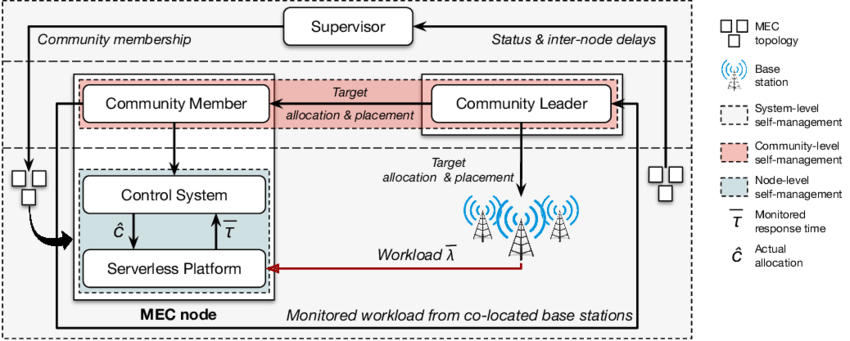
\includegraphics[width=\textwidth]{StructurePAPS.png}
    \label{fig:structure}
    \caption{PAPS general structure}
\end{figure}

\subsubsection*{System level}
Since MEC topologies can be really large and densely connected, the first step is to \textit{partition}
the network in multiple delay-aware sub-networks called \textit{communities}. Each community
is composed by a set of nodes whose propagation delay from one another is below a given 
threshold. PAPS assumes the availability of a \textit{supervisor} that has a global view of
the MEC topology and uses the SLPA \cite{SLPA} algorithm to create the communities.
\par
SLPA is an algorithm which uses label spreading techniques to decide to which community each node will belong.
It is composed of a variable number of iterations (stable solutions are obtained with 20) where nodes spread their labels 
around to their neighbors.
The main component of this  algorithm is the memory inside each SLPA node, in which it will store all the labels received.
\\
In each iteration, all the nodes will become one at a time 
\textit{listener} and will collect a label, selected from the memory, from any nearby 
node (\textit{speaker}). Once all the labels are collected, the listener selects the 
most popular node (or selects a node with any other listening rule) and adds it to its
memory.
An iteration ends when all the nodes have been listener once. \\
Since the initial idea of this 
algorithm was developed to divide social networks profiles in communities, it can create 
overlapping node which will belong to more than one community. 
In PAPS a node that is a member of multiple communities will have to balance its resources in order to address
the requests coming from different community leaders.
Each community will
elect a \textit{leader} which will be in charge of managing the community and the communication
between the nodes.

\begin{figure}[h]
    \centering
    \subfloat[SLPA Pseudocode]{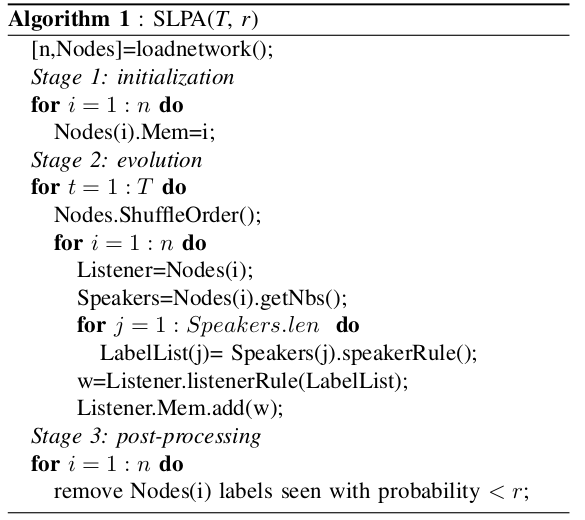
\includegraphics[width=.4\linewidth]{SLPAPseudocode.png}}%
    \label{fig:pseudocode}
    \subfloat[An example of communities division]{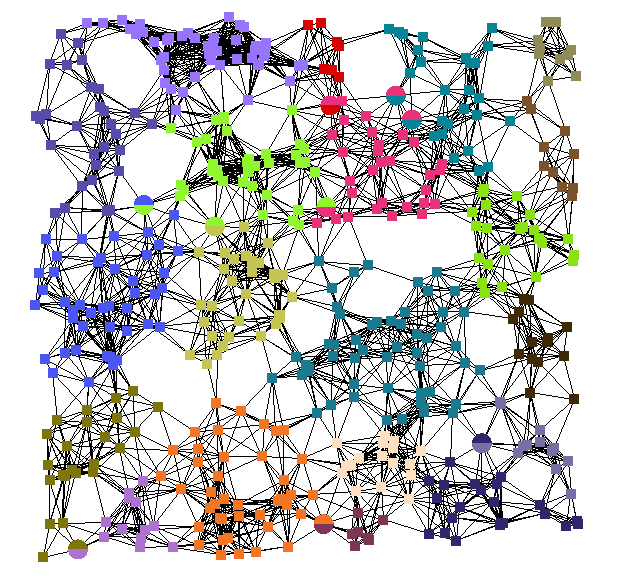
\includegraphics[width=.4\linewidth]{PPAP_communities.png}}
    \label{fig:communities}
\end{figure}

\subsubsection*{Community level}
Communities aims to minimize the likelihood of SLA violations so that the MEC nodes
can operate under feasible conditions.\\
A community leader has to supervise its community, by ensuring that every node it's still up and running.
A heart-bit signal for each node is checked inside the community.
Each community leader will manage the \textit{allocation and placement} phases by looking at 
the aggregate demand to each service and the node capacities in order to decide how to 
distribute resources among the nodes in its community. This is done solving a \textit{mixed
integer programming (MIP)} problem whose goal is to minimize the overall community delay. 
The MIP is solved periodically by the community leader which will then contact the other members
to communicate the new configuration.
Informed load balancers will use the information contained in this plan to route the workload 
coming from different base stations to the actual destination.

\subsubsection*{Node level}
The Node-Level Self-Management system aims to keep the response time for a given function fixed, 
by deploying and removing containers accordingly to the measured workload.
In order to achieve this, every node has a controller for each function that is hosting; all the controllers
run in parallel and independently.
Each controller accepts as input the number of container allocated for its function and the 
measured arrival rate, and outputs the response time. The objective is to keep the response time
at the control set point, which must be lower than the SLA.
\\
\\
Currently PAPS is a prototype that works on a simulated network in PeerSim \footnote{http://peersim.sourceforge.net/},
in which the serverless functions are implemented as java threads. The prototype runs on a single machine and simulates
the workload by drawing from a set of probability distributions.
The goal of our project is to integrate PAPS with real world frameworks, in order to test and have a better
idea about the feasibility of this project on a real multi-node environment.




%------------------------------------------------------------------------------------------------------------------------------------------------
{{\section{Research}\label{sect:research}}}
%introzioncina su cosa sono sti framework
%framwrok serveless vanno bene così.
%ampliare funzionamento di kubernetes e magari spostare come 
%implementiamo noi le labels in implementazione 
%OSCAR
\subsubsection*{Framework research}
% Il problema di questi framework è che comunque nascono l'infrastruttura sottostante e la
% gestiscono loro sotto, dando un accesso solo tramite API in maniera limitata.


Since PAPS focuses on serverless function, initially the research looked for a framework 
that would allow the user to create in a immediate way functions and would give the opportunity to manage their
deployment and placement inside the network.
In this way, the creation of containers is sped up, because the framework automates all the process
of creating a container and eliminates the need of adding useless boilerplate code.
\par
The first candidate was OpenWhisk \footnote{OpenWhisk website: https://openwhisk.apache.org/}, a serverless platform able to run 
functions on top of an existing infrastructure. The idea was to integrate it on top of a Kubernetes 
cluster, running a series of docker \footnote{Docker website: https://www.docker.com/} containers. \\
Searching on the internet information about the integration of those platforms, other two 
options were available: OpenFaas \footnote{OpenFaas website: https://www.openfaas.com/} and 
Kubeless \footnote{Kubeless website: https://kubeless.io/}. For what concerns 
the functionalities the three frameworks are pretty similar one to another.
They all provide a mechanism to deploy functions that can be written in various programming languages.
These functions accept arguments and give a response in the form of a json file, whose structure
is determined by the programmer. In this way the mechanisms that deploy and call the functions are language agnostics.
\par
Function calls are controlled with Triggers, components that reacts to certain events inside the 
ecosystem (such as HTTP request or the call of another function).
OpenWhisk offers a very detailed protocol on how to design triggers, functions, and rules
that connect these two elements.
On the other hand, OpenFaas is less focused on this functionality and more oriented on HTTP calls.
\par
Kubeless stands out since it has a built-in synergy with Kubernetes. In order to support the creation of functions, 
it extends the Kubernetes API by creating a CustomResourceDefinition, a RESTful resource that is saved inside the Kubernetes
system. This new type of resource can be accessed like any other normal object inside Kubernetes
by making REST calls (via CLI or HTTP request).

\par
The main issue with OpenWhisk and Kubeless is 
that they are written in Scala and Akka; OpenWhisk also has a complex structure and for that reason 
is not optimal for a project like this. For what concerns OpenFaas, it is written
in Go and offers some additional features like a metrics system and the possibility to 
customize the scheduling policy used by the framework.
\\
During the research process one main  problem came out: all the frameworks hide to the final user 
the underlying infrastructure, making the integration of PAPS functionalities hard.
To solve this issue, the best decision was to build something directly on top of Kubernetes
using the provided API, available for a large variety of languages, to create, manage and 
delete containers when needed. \\
For what concerns the framework, OpenFaas came in handy to provide a frontend module 
useful for PAPS users which will be easily able to upload the functions that PAPS
will manage and distribute. We chose OpenFaas since it offers both a
simple UI and the possibility to be managed by a CLI. It was also the only one that offered the possibility to 
install a statistics collection module, which can be used to monitor how the
system is working in a real environment.


\subsubsection*{OpenFaas}
OpenFaas is a serverless framework that does not manage the infrastructure, since it delegates
this task to other IaaS frameworks (such as Kubernetes).
It works at the application level, easing the creation, management and deployment of functions
on the cluster. 
\par
A function is a piece of software that provides some functionality, receiving request and sending response
in a json file format. It will be deployed in the cluster in the form of multiple containers,
on which the user has no direct control or knowledge.
This allows the user to have a high level view of its functions, without having
to worry about the complexity of the management of the infrastructure, since functions and containers are decoupled.
\par
For what concerns the architecture, the main component of OpenFaas is the \textbf{API-gateaway}.
It exposes the REST-API that allows the user to manage its functions.
Both function calls and management requests are sent to the gateaway, which in turn will provide
to contact the right component in order to perform the desired action.
The API-gateaway can be invoked via CLI, UI or HTTP requests.
\\
When a function is deployed, on or more pods/containers are created. The \textbf{WatchDog}
is the component that is responsible for starting and monitoring functions. It becomes
an init process with an embedded HTTP server, and can support concurrent requests, timeouts and
healthchecks.
\\
The \textbf{Alert Manager} controls the traffic to which the function are subjected.
This is done monitoring the metrics produced by Prometeus. When the current configuration
cant keep up with the current workload or too much containers are allocated, the Alert Manager
fires an alert to the API-gateaway, that will provide to change accordingly the number of containers.
\\
All these components are builded on the cluster as standalone containers, and so they can be also
duplicated depending on the cluster administrator needs.

\subsubsection*{Kubernetes integration}
Kubernetes is an orchestration framework that automates deployment, scaling and management of containerized
applications on a multi-node cluster.
The containers are bundled in particular entities, Pods, that contain all the dependencies and 
additional metadata about the deployment. A set of controllers allows the user to automate
in a flexible way the deployment of these pods.
\\
Kubernetes offers to the user REST API, through which all object can be created, read, updated
and deleted. This object are stored inside the system and describe the desired state of the cluster.
\\
All objects have a metadata field, in which labels can be added and removed.
Labels can be used to mark an object, and their meaning is defined by the programmer that created it.
Labels allows filtering while asking for resources, and so they can be used to assign a particular role 
or attribute to a certain object.
\par
The infrastructure is managed with the help of some key components, that are divided into two categories:
Control Plane components and Kubernetes Node components.
\begin{figure}
    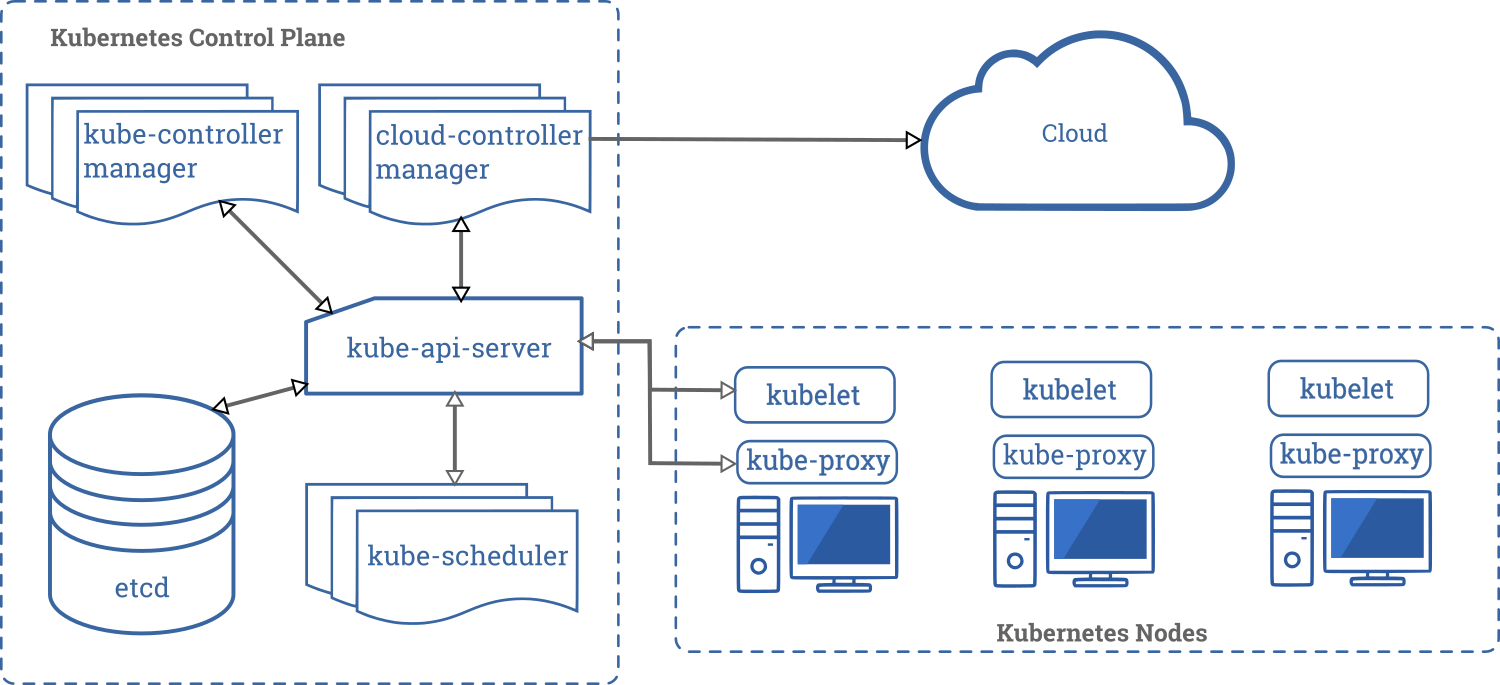
\includegraphics[width=\linewidth]{Images/components-of-kubernetes.png}
    \caption{Components of Kubernetes.}
    \label{fig:boat1}
  \end{figure}


The \textbf{Control Plane components} has the role of managing the cluster, by making global decisions.
It detects and responds to cluster events. These components can be run on any machine, but usually
they are placed on a node called Master.
The \textbf{kube-api-server} is the frontend for the Kubernetes Control Plane. It implements Kubernetes'
REST API, that can be accessed with a CLI or an HTTP request. It allows to create and manage resources,
giving fine grained information about the cluster.
\\
The \textbf{etcd} is a key-value based storage, in which all the data about the cluster are saved.
\\
The \textbf{kube-scheduler} is notified when a pod has been created. Its function is to place this pod
on a node, taking into account some factors such that individual and collective resource
requirements, hardware/software/policy constraints, affinity and anti-affinity specifications,
data locality, and inter-workload interference.
The default scheduler can be replaced with a custom scheduler. A schedule routine
is composed of two phases. The \textit{Filtering} phase has the objective to identify a set 
of candidates nodes on which the pod can be scheduled, while in the \textit{Scoring} phase
a score for each node is calculated with the help of some heuristics. The node with the highest score
is the one that will host the given pod.
This two phases are ignored if the current pod has already specified in its fields the node
in which it will be scheduled.
\\
The \textbf{kube-controller-manager} runs all controller processes that manage both nodes and 
pods. The \textit{Node controller}
checks the status of the nodes in the cluster, responding accordingly if a node fails.
The \textit{Replication controller} controls all the pods, and reacts to changes of the pod number
by allocating or de-allocating accordingly to the desired state and the workload. If a node fails, all 
the pods that were active on it will be placed again thanks to its routines.
\par 
The \textbf{Kubernetes Node components} are placed on the node of the cluster and handle
the real creation and destruction of the containers.
\textbf{Kubelet} makes sure that containers are running in a Pod. It receives from the kube-api-server
a PodSpec (an object that describes all the dependencies and characteristics of the pod that
will run on the node) and checks if the containers described are running and healthy.
Kubelet does not manage containers that have been created outside of Kubernetes.
\\
The \textbf{kube-proxy} allows nodes to communicate with the api server. It maintains network rules,
allowing pods to communicate with one another.
\\
The \textbf{Container Runtime} is the software responsible for running containers.




%------------------------------------------------------------------------------------------------------------------------------------------------
\clearpage
{{\section{General Implementation Idea}\label{sect:generalImpl}}}
%come vorremmo fare noi Partition, Allocation e Placement
%FABIO
Thanks to the results of the research phase, we decided to use mainly kubernetes functionalities
and extension possibilities to implement PAPS phases and use OpenFaas as a frontend module to 
allow an easy deployment of the serverless functions.
\begin{figure}[h]
    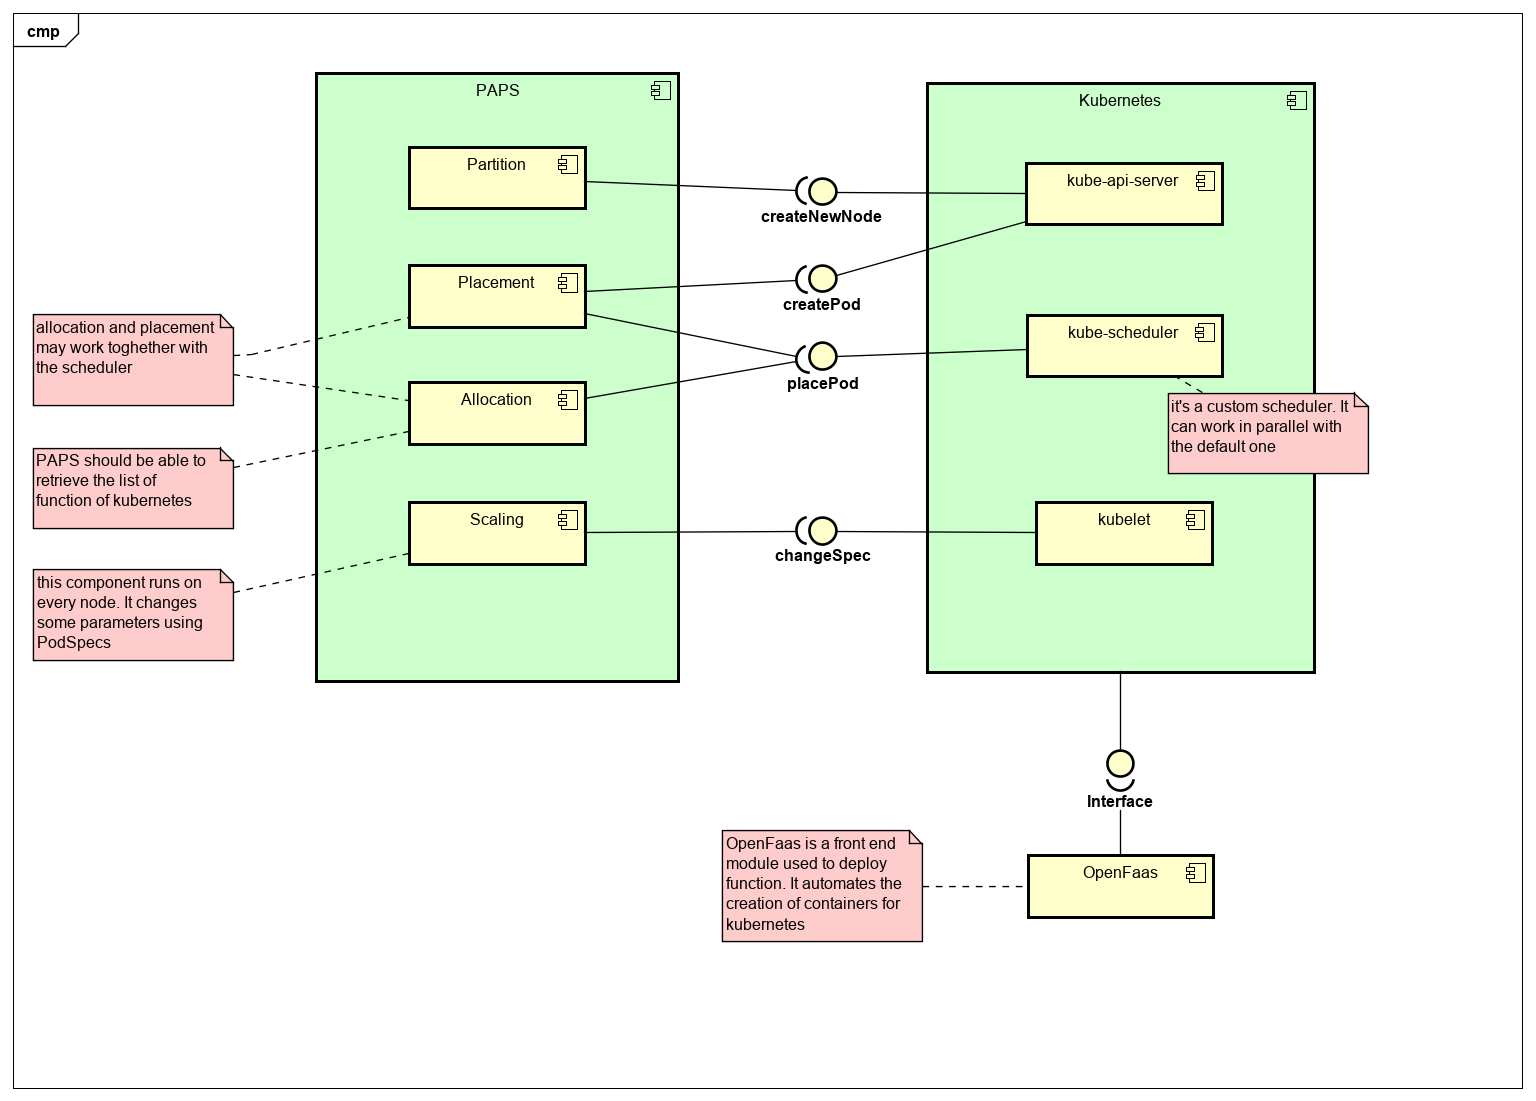
\includegraphics[width=\textwidth]{componentPAPS.png}
    \label{fig:component}
    \caption{Component diagram of PAPS}
\end{figure}

The first of the four PAPS phases is the \textbf{partition}, in this phase the original 
network topology on which PAPS will need to work is divided into delay-aware communities in 
order to reduce the scope of the following parts. To do that the idea is to take as input a 
delay matrix describing the measured delay between the nodes of the networks and other 
additional parameters that can be useful to describe the desired behavior of the partitioner.
This input can be provided as a file input or even through the OpenFaas GUI and will than be
parsed by the program to fill some data structures. The partition will first of all connect to 
kubernetes API manager and do a call to obtain the list of registered nodes to check if they 
match with what has been parsed from the input. This operation needs to be done in order to
avoid the presence of nodes in the topology that are not actually managed by kubernetes and 
so that can't be modified and labeled according to the specific needs. 
%------------------------ descrizione slpa da spostare
To divide the network the partition will use SLPA, an algorithm which uses label spreading 
techniques to decide to which community each node will belong. The main component of this 
algorithm is the memory inside each node, there it will store all the labels received and 
it will process them in each round to decide the label to spread and at the end of the 
process the final label which will identify the community. Since the initial idea of this 
algorithm was developed to divide social networks profiles in communities, it can create 
overlapping node which will belong to more than one community. 
%-------------------------- 
For our implementation this
is a problem but can be easily solved in many ways. Since all the labels kept at the end 
of the process are valid ones the simplest idea is to just randomly choose one of them or,
with some more processing, is also possible to pick the most popular one among all the 
remaining labels. In our implementation we select the first one in the list, which is 
equal to picking a random one since all the nodes are shuffled at each round, but it can 
be easily changed by changing few lines in the SLPA code.


As an additional division tool the Partition keeps the size of the communities under control
applying Round Robin to oversized communities to split them in smaller ones and have all 
communities under a given threshold size.\\
The Kubernetes label feature can be used to perform the partition of the network.
Every Node can be marked with two labels, "COMMUNITY" and "ROLE". The former assigns to the node 
the PAPS community to which it belongs, while the latter specifies if the host is the leader of the
community or just a member that executes the leader's allocation plan.
By filtering on these labels, all the nodes of a community can be retrieved, easing the tasks performed 
by the Allocation and Partition modules.
\\

Once the network is split in communities, in each one the \textbf{allocation} phase will take
place. There the community leader will compute the resource allocation to assign to each node
according to the current load of the network and to respect the SLA of each function deployed.
To do that a MIP model is solved internally, using the IBM solver \footnote{IBM ILOG CPLEX 
Optimization Solver: https://www.ibm.com/products/ilog-cplex-optimization-studio}, stored in 
a dedicated container inside the leader node. Since it is inside the community leader, it 
will need to have access to some performance metrics regarding the other nodes of its community
and this can be easily done through the kubernetes API by filtering with the correct community
label. The result of the allocation will tell how many pods of each function will be scheduled
on each node in order to meet the SLA for all the received request at that moment.
The allocation phase will be periodically triggered to check if the provided allocation
schema is still valid or needs to be changed. \\
All the nodes will also implement an internal allocation phase which will change the amount 
of resources assigned to each scheduled pod inside the node itself since between two 
allocation cycles the amount of resources needed to meet the SLA of each function will 
slightly change. To do that a pod for the allocation will be always deployed in each node
and it will contain a function which works only on local resources.\\

The allocation phase will work in combination with the \textbf{placement} phase using a
\textit{kube-scheduler} module to actually deploy the pods necessary to realize the 
computed model. The kube-scheduled will be a custom module running in the network and will
contain some rules on how to deploy pods according to the MIP result. To correctly schedule 
pods, the filtering rules of the scheduler will be modified to filter by community and for 
a particular node in the community. Once the correct node is identified, the scheduler will 
actually deploy the pod in the node and from now on it will be up and running and ready to 
be used. \\

The last phase is the \textbf{scaling} which will use a PID controller to keep meeting the
SLA of all the functions on each node. Since this is a node level function, it will be
deployed in a pod on each node, maybe together with the allocation part, and will be always
up to check the resource utilization. This part will trigger the kubelet module of kubernetes
by changing the PodSpec relative to the deployed function if needed to keep the performance
under the given SLA. If a more drastic change is identified, it will make a call to the 
leader and ask for a new MIP evaluation even before the normal control period. 






%------------------------------------------------------------------------------------------------------------------------------------------------
\clearpage
{{\section{Partition Implementation}\label{sect:implementation}}}
%aggiungere immagini
The scope of this project is to develop the first of the four PAPS phases: the network 
partitioning. This part of the framework has the role of dividing the network into 
delay aware communities in order to reduce the number of nodes on which the next phases
will need to work. The first piece needed to partition the network is the network itself:
it will be provided as an input in the form of a delay matrix, from a node to any other
node, and the number of nodes which are part of that network. \\ 
Once the input is parsed and data are acquired, the program checks if the nodes specified 
in the input are really present in the cluster. To do that the program interrogates 
Kubernetes, through a call to the API, to obtain the list of objects (V1Node) related to
all the nodes registered in the cluster and checks if the names given in the
input matches with real cluster nodes. If all the matches are positive, each selected 
node is wrapped in a SLPA \cite{SLPA} node to allow an effective partition of the network.
This wrapping adds to the initial Kubernetes structure a memory and a list of nearby 
nodes and a label which it will try to spread. To understand why those structures are 
added, a brief introduction on SLPA is needed. It is composed of a variable number of 
iterations (stable solutions are obtained with 20) where nodes spread their labels 
around to their neighbors. In each iteration, all the nodes will become once 
\textit{listener} and will collect a label, selected from the memory, from any nearby 
node (\textit{speaker}). Once all the labels are collected, the listener selects the 
most popular node (or selects a node with any other listening rule) and adds it to its
memory. When it will become speaker it will select a label from its memory according 
to a probability distribution based of the number of occurrences of each label in the 
memory. An iteration will end when all the nodes have been listener once. \\
After the given number of iterations, the memory of each node will be post-processed, 
the most popular node in the memory will determine its community. In case of multiple
labels with the same number of occurrences, the node will be assigned to multiple 
communities and will be considered an \textit{overlapping node}. Since PAPS doesn't 
want to deal with those kind of nodes, the overlap will be solved selecting randomly 
one of the overlapping communities. \\
With this procedure the network will be effectively divided into communities but, 
to keep the size even more under control, oversized communities will be split to better
fit the size limit (also provided as input). \\
Now that all the nodes are assigned to a community, another API call will modify the
existing node that will add a label in order to easily recognize and manage each community.





%------------------------------------------------------------------------------------------------------------------------------------------------
\clearpage
{{\section{Conclusion}\label{sect:conclusion}}}
%limiti attuale lavoro
%direzione in cui andare
%OSCAR
Our work focused mostly on finding the best frameworks that would support PAPS functionalities.
These serverless computing frameworks turned out to be excellent tools for the production
and deployment of stateless functions, but they also had evident limits in managing the underlying
infrastructure.
Since we needed a much lower level of abstraction, we decided to use also Kubernetes and extend
its functionalities, taking advantage of its modular architecture.
We implemented the Partition module on Kubernetes, and we think that the remaining modules will
be placed here as well. In this way, OpenFaas has the role of a frontend module, that allows
the user to upload its function in the cluster without having to care about the infrastructure.
We chose OpenFaas for its excellent support and simplicity, but it can be substituted with other frameworks
with very little effort, since PAPS works at the Kubernetes level.
PAPS is mostly focused on a workload that come from outside the MEC network, and so the trigger functionality,
that links the execution of multiple functions, was very marginal.
If a future work will focus on a micro-services architecture, OpenWhisk may be
a better option, since it offers a cleaner and more powerful structure for this mechanism.
\par
For what concerns the implementation of the Partition module, we decided to write ourselves 
the SLPA algorithm, and we used a round robin approach to break down too large communities.
This part of the component could be substituted by using the GANXiS \footnote{GANXis: https://sites.google.com/site/communitydetectionslpa/} software, a program
that runs the same algorithm and has more complex and effective techniques to reduce
the size of the communities inside the given boundaries.
The next step in the development of PAPS will have to be the implementation of the Allocation 
and Placement components. Their functioning is completely decoupled from the Partition module,
since they just need to know the structure of the communities, and any change in its logic
will have no effect on how the container will be disposed inside the cluster.
Kubernetes offers very powerful tools that allows to schedule and place pods on the nodes of the cluster,
while taking care that every container is healty and running. Thanks to this functionality,
the Allocation and Placement will just have to produce an allocation plan without having to
care how to enforce it.



%------------------------------------------------------------------------------------------------------------------------------------------------
\clearpage
{{\section{References}\label{sect:biblio}}}
\begin{thebibliography}{9}
    \bibitem{PAPS}
        Baresi, L., Mendonça, D., Quattrocchi, G.: 
        \textit{PAPS: A Framework for Decentralized Self-management at the Edge.}
        In: Service-Oriented Computing, pp.508-522, (2019).   

    \bibitem{SLPA}
        Xie, J., Szymanski, B K, Liu, X.:
        \textit{SLPA: Uncovering Overlapping Communities in Social Networks via
        A Speaker-listener Interaction Dynamic Process.}
        In Proc: Data Mining Technologies for Computational Collective 
        Intelligence Workshop at ICDM, Vancouver, CA pp. 344-349, (2011)

    \bibitem{Edge}
        Shufen Wang:
        \textit{Edge Computing: Applications, State-of-the-Art and Challenges, Advances in Networks.}
        Vol. 7, No. 1, pp. 8-15. doi: 10.11648/j.net.20190701.12 (2019)

    \bibitem{Kube}
        https://kubernetes.io/

    \bibitem{Docker}
        https://www.docker.com/

    \bibitem{OpenWhisk}
        https://openwhisk.apache.org/

    \bibitem{Faas}
        https://www.openfaas.com/

    \bibitem{Kubeless}
        https://kubeless.io/

    \bibitem{GANXis}
        https://sites.google.com/site/communitydetectionslpa/    

\end{thebibliography}




\end{document}